% Appendix A
\chapter{XBee join and send time experiments} % Main appendix title
\label{AppendixA} % For referencing this appendix elsewhere, use \ref{AppendixA}
\lhead{Appendix A. \emph{XBee join and send time experiments}} % This is for the header on each page - perhaps a shortened title
\section{Distance relation test}
This table contains the results of two different test programs (blue and green values). The program scenario is as follows:\\
\begin{enumerate}
\item Turn on Waspmote and XBee
\item Wait until XBee has joined
\item Measure battery level, temperature, humidity and pressure (each with 100 milliseconds delay between samples)
\item Send the values and turn off Waspmote
\end{enumerate} 
\hspace{1cm}
\begin{figure}[htbp]
\centering
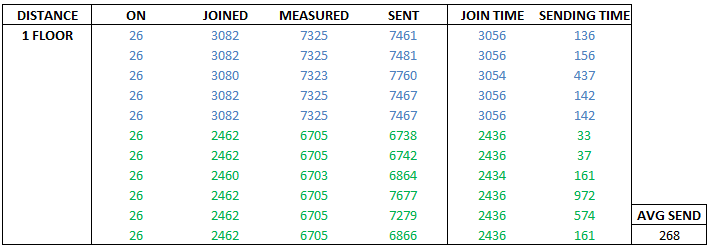
\includegraphics[height=5.5cm]{floors1}
%\rule{30em}{0.5pt}
%\caption[XBee join and send times: distance relation]{Measurements of join and send time at different distances.}
\label{fig:floors1}
\end{figure}
\begin{figure}[htbp]
\centering
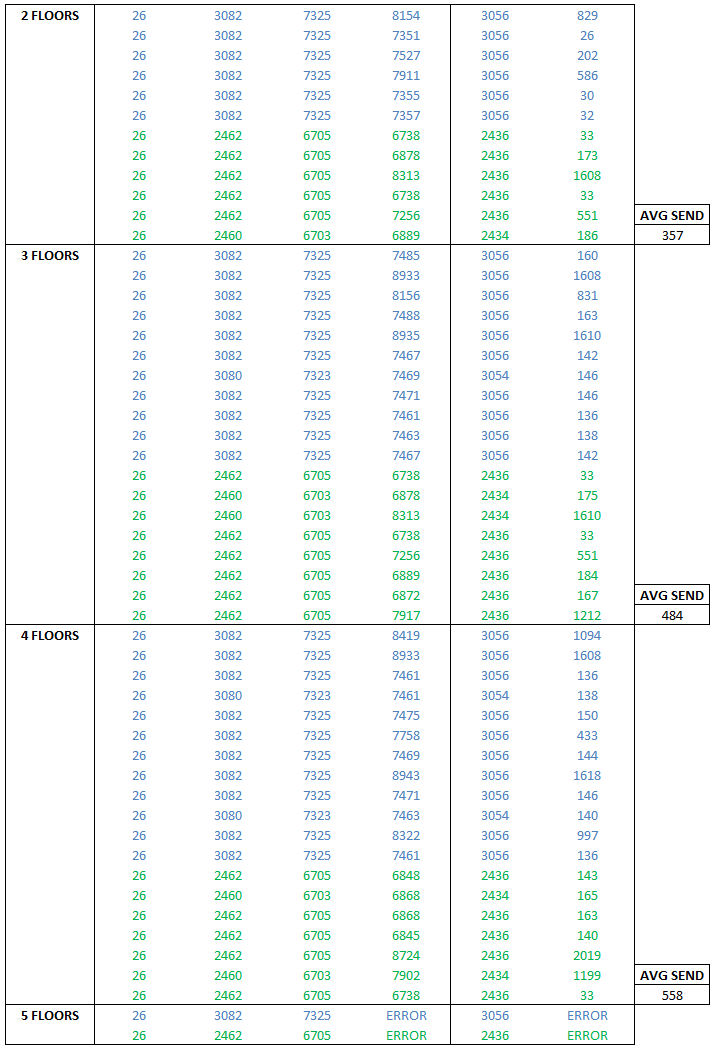
\includegraphics[height=23cm]{floors2}
\rule{30em}{0.5pt}
\caption[XBee join and send times: distance relation]{Measurements of join and send time at different distances}
\label{fig:floors2}
\end{figure}\\

\section{First time reduction}
The next results are obtained via the following scenario:
\begin{enumerate}
\item Turn on Waspmote and XBee
\item Measure battery level, temperature, humidity and pressure (each with 100 milliseconds delay between samples)
\item Check XBee association
\item Send the values and turn off Waspmote
\end{enumerate} 
It appears that when the XBee has been on for a sufficient amount of time, the time to request the node's association state is constant at about 450ms.\\
A second conclusion is that without obstacles and with a node that already is joined a while before trying to send leads to a constant sending time.\\  \bigskip \bigskip
\hspace{5cm}
\begin{figure}[htbp]
\centering
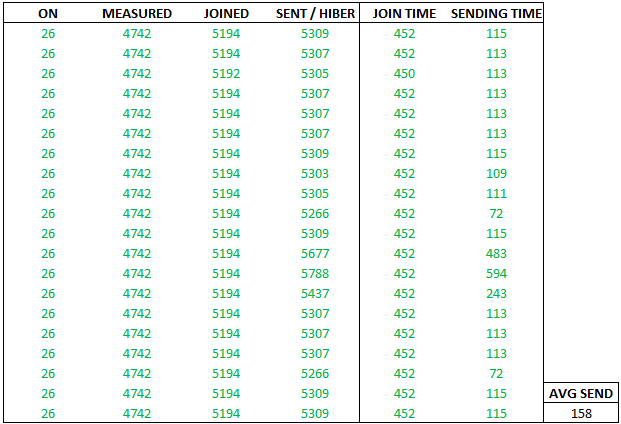
\includegraphics[height=10.5cm]{floors3}
%\rule{30em}{0.5pt}
\caption[XBee join and send times: first time reduction]{XBee join and send times: first time reduction}
\label{fig:floors3}
\end{figure} 
